
\Chapter{Eszközkészlet és tervezés}
\Section{Rendszer követelmények}

\subsection{Általános leírás}
Egy olyan elosztott rendszer létrehozása a cél, ami képes a drónszállítás közben keletkező valóságnak megfelelő adatokat szimulálni és hatékonyan feldolgozni.
Ezeknek az adatoknak a feldolgozását vizsgálom, több kontextusból.
Egyrészt a hálózaton való kommunikaáció hatékonyságát vizsgálom, tehát hogy mennyi adatforgalommal jár a kommunikáció, mennyi erőforrással jár csak a kommunikáció a küldő és fogadó részéről (tehát a feldolgozás nélkül).
Másrészt azt, hogy milyen hatékony az kommunikációval közölt adatok feldolgozása, azaz a hálózaton használt adatformátum átalakítása a programban használt formátumra. Másrészt összehasonlítjuk az adatbázisba való mentés hatékonyságát.
Mivel elosztott rendszerekről van szó, nem egy darab program lesz.
Mikro-szervízhez hasonlóan működnek majd a programok.
Ez azt jelenti, hogy ha 100 adat feldolgozást végző program fut egy terhelést elosztó proxy mögött, akkor ugyanolyan viselkedés várható mint ha csak 1 program futna.
A drón szenzorai által gyűjtött adatokat telemetria adatoknak nevezzük. A programok egy részének ezeket az adatokat kell tudnia generálni, egy másik részének feldolgoznia.

\subsection{Hatékonyság}
A hatékonyság alatt egyszerre értjük a teljesítményt, tehát hogy mennyire gyors a feldolgozás, és azt is hogy ez a feldolgozás mennyi erőforrást használ.
Mindezt úgy kell elérnünk, hogy az  adatok feldolgozása aszinkron módon történik, de az aszinkron feldolgozás nem járhat lényeges többletmunkával és semmilyen módon nem akadályozhatja a rendszer megfelelő működését.
Tehát fontos, hogy jól használjuk ki az erőforrásainkat, és a rendszer bármikor skálázható legyen horizontálisan is.


\subsection{Funkcionális követelmények}
A szimulációban többféle protokollt és adattovábbításra használt formátumot hasonlítunk össze, így a programot úgy kell felépíteni, hogy ki lehessen cserélni ezeket részket anélkül hogy a program üzleti logikájának működését befolyásolnánk.
Az adatközpontok és drónok közötti telemetria adat kommunikációt és annak feldolgozását összehasonlítjuk egy HTTP 1.1 -en műkodő JSON adatformátumot használó REST~\cite{Wikipedia-REST} API-n, egy HTTP 2 -n futó gRPC-t használó végponton is.
Az adatok mentését is több adatbázison kell tesztelni, így az adatbázisnak is cserélhetőnek kell lennie.

%TODO: ide még írni
\Section{A Go nyelv áttekintése }

A Go program nyelv, (sokszor Golangként emlegetik) egy nyílt forráskódú modern programozási nyelv melyet a Google fejlesztett ki.

A Google-nél olyan problémák adódtak, hogy a konkurrenciát nem tudták megfelelően kezelni a még eredetileg
1 processzoros számítógépekre kifejlesztett nyelvek, mint a Java, C++.

Persze azóta sokat fejlődött ezen nyelvek konkurrenciakezelése de nem tudnak versenyezni a Go-val
ha a gépi és fejlesztői hatékonyságot is figyelembe vesszük.
Probléma volt az is, hogy ezeknek a nyelveknek nagyon nagy a fordítási idejük. A 2000-es évek végén ez azt jelentette
hogy egy Java vagy C++ program a Google-nél 1 hét alatt fordult le, csak hogy ki tudják próbálni.
A nyelvek bonyolultságával is baj volt, ahogy fejlődtek a nyelvek egyre nehezebb volt egy régi programot tovább fejleszteni,
illetve új programozóknak megtanulni a nyelvet.

Hogy ezeket a problémákat orvosolják, a Google a legjobb tervezőket hívta össze, hogy együtt alkossanak egy új nyelvet.
Így született meg a Golang.
A fejlesztést olyan szakemberek vezették, akik korábban a Unix operációs rendszer, a Java HotSpot JVM
vagy az UTF-8 karakterkódolás fejlesztésében is kulcsszerepet játszottak.
Például Ken Thompson, Rob Pike és Robert Griesemer.

A cél az volt, hogy régebbi általános célú nyelvek hiányosságait kiküszöböljék, és csökkentsék a bonyolultságot,
hiszen a megváltozott üzleti és technológiai körülmények között ezek a nyelvek nem bizonyultak elég hatékonynak.
Nem várhatták el hogy egy friss diplomás hatékonyan kezeljen egy olyan ''felpuffadt'' nyelvet mint a Java.

A felhőben való futtatásra olyan alkalmazások készítésére volt igény, amelyek nagy hatékonysággal futnak és kiválóan skálázódnak.
A végeredmény egy olyan nyelv amely általános célú, könnyen tanulható, kifejező, tömör, letisztult és hatékony.
Éppen ezért kiválóan alkalmazható ott, ahol a kódbázishoz nagyszámú, gyakran cserélődő, változó összetételű programozói gárda fér hozzá,
akár időben és földrajzi elhelyezkedésben is megosztva.

Szintaktikailag a C-hez hasonlít de nagyon könnyen tanulható nyelv.
A legnagyobb újítás a konkurrencia mechanizmus (főleg a saját ütemező) és hibakezelés körül volt.
A Go konkurrencia mechanizmusa megkönnyíti olyan programok írását amelyet a legtöbbet hozzák ki a többmagos és hálózaton összekötött gépekből.
Gyorsan lefordul gépi kódra de rendelkezik garbage collection-el és runtime reflection is van beépítve.
Gyors, statikus nyelv de úgy érezzük mintha egy dinamikus futás időben fordított nyelv lenne.
Tartalmaz \textit{race detector}-t is ami nagyon fontos egy ilyen nyelvben, mert fel tudja ismerni a konkurrens/párhuzamos programozásnál felmerülő gyakori problémákat.
Mivel nagyon jól kihasználja a gép erőforrásait és a hálózatot manapság a felhőben futó kódok nagyrésze Go.
Idézet egy cikkből \cite{HWSW}:
Beszédes, hogy a Linux Foundation által létrehozott Cloud Native Computing Foundation (CNCF) keretein
belül támogatott projektek nagy része Go-ban íródott, többek között a Kubernetes, a Prometheus, az Istio, de ebben írták a Dockert is.


\subsubsection{A Go konkurrencia mechanizmusa}
A konkurrencia a nyelv alapjának része. A 3 legfontosab dolog ebből a szempontból az hogy a Go-nak saját ütemezője van,
a gorutinok (''goroutine'') és csatornák (''channel'').\\
A goroutin egy szójáték a hasonló coroutine-al. A lényege hogy ezek a folyamatok a Go runtime-on belül futnak, sokkal kisebbek mint egy processz, megabájtok helyett csak pár kilobájt,
így pillekönnyűnek számítanak az Operációs rendszer processzeihez képest. \emph{Egy programban akár több millió gorutin is futhat egyszerre!}
A saját ütemező (scheduler) sokkal hatékonyabb mintha csak létrehoznánk egy processzt és hagynánk hogy az Operációs rendszer ütemezze,
mivel így az ütemező meg tudja határozni hogy az adott gorution milyen állapotban van (várakozik, futtatható, vagy fut) és hatékonyabban tudja
kiosztani az erőforrásokat. Értelemszerűen például egy blokkoló, épp I/O műveletet végző gorutint nem fog futtatni hanem helyette más gorutinokat részesít
előnyben. De fontos hogy az ütemező nem determinisztikus, így nem tudjuk előre megmondani melyik gorutin fog következni.\\
4 féle esemény fordulhat elő a Go programokban ami miatt az ütemező döntéseket hozhat:
\begin{itemize}
    \item A \emph{go} kulcsszó használata
    \item Garbage collection
    \item Rendszer hívások
    \item Szinkronizálás és orchesztráció, vezérelés
\end{itemize}
A \emph{go} kulcsszó használata: \par
A go kulcsszó létrehoz egy új gorutint, így az ütemezőnek lehetősége van beavatkozni.\\
Szinkronizálás és vezérlés: \par
Ha egy atomi, mutex, vagy csatorna művelet, függvényhívás miatt egy Gorutin blokkolni fog, az ütemező kontextus cserével egy másik gorutinnak adhat erőforrást. Ha a blokkolt Gorutin újra futtathatóvá válik, sorba állítja az ütemező és végül visszakapja az erőforrást.\\
A gorutinok ugyanabban a címtérben futnak, ezért a megosztott memóriához való hozzáférést szinkronizálni kell.

A csatornák a típusos vezetékek amelyeken adatokat küldhetünk és fogadhatunk a csatorna operátorral, <-.
Az adatok a nyíl irányába folynak. Ahhoz, hogy jobban megértsük a csatornák szükségességét meg kell értenünk a következő, a Golang tervezői szerint információmegosztásra megfelelő konkurrencia modellt:
\emph{''Do not communicate by sharing memory; instead, share memory by communicating.''}
Tehát arról van szó, hogy ha direkt megosztott memórián keresztül kommunikálunk abból csak baj lehet, a megosztott memória ilyen használata veszélyes, helyette egy olyan módszert
kell alkalmazni ami védelmet biztosít a megosztott memória felett. A Golang csatornái pont ezt az elvet követik.
\begin{python}
    ch <- v    // Snd v to channel ch.
    v := <-ch  // Receive from ch, and
    // assign value to v.
\end{python}
Alapértelmezett beaállítás szerint a csatornák blokkolnak amíg az egyik oldal küld vagy fogad.
Ez lehetővé teszi a szinkrinizációt anélkül hogy zárakat vagy feltétel változókat hoznánk létre.

Bufferelt csatornák
\begin{python}
    ch := make(chan int, 100)
\end{python}


\subsubsection{A Go hibakezelése}
A hibakezelés nagyban megváltozott azzal hogy a Go-ban nem try és catch blokkba zárjuk a hibára futható programkódot
hanem van egy beépített hiba típus, ami a függvények visszatérési értéke lehet. Fontos tudni, hogy a Go-ban egy függvény többféle
visszatérési értékkel rendelkezhet. Ha nem egy nagyon egyszerű programot fejlesztünk, a legtöbb függvényünk utolsó visszatérési értéke egy hiba típus lesz.
Csak az olyan atomi műveleteket végző függvényeknél nem szoktunk hiba típust használni ami biztos hogy nem fut hibára normális körülmények között.
Például egy függvénynek ami összeadásokat, vagy egyéb egyszerű műveleteket végez értelemszerűen nincs értelme hogy hibával térjen vissza.
De egy olyan függvénynek ami egy fájlt nyit meg, már van értelme hiba típussal visszatérnie, mert több hiba is előfordulhat az instrukciók futása közben, lehet nem létezik a fájl, vagy nincs jogosultságunk megnyitni.
\begin{python}
    func Open(name string) (file *File, err error)
\end{python}
A fenti függvény például egy Fájl típus pointerét és egy hiba típust ad vissza. Ha nem futott hibába a program, az err változó nil értéket kap.

Tehát egy hiba kezelése például így nézhet ki:
\begin{python}
    file, err := Open(''fajlnev'')
    if err != nil {
        log.Println(err)
        return nil, err
    }
\end{python}

Ennek a hibakezelésnek az előnye, hogy a hibák mint visszatérési értékek buborékként felpezsegnek a függvényhívásokon keresztül.
De a programokban amiket fejlesztünk célszerű saját hiba típusokat létrehoznunk rétegenként, vagy legalább az üzleti logika rétegben. Ez jó a kód átláthatóságához,
az esetleges hibakereséshez (debugging) elengedhetetlen. Ezen kívül fontos hogy az alkalmazásunk nyitott részén ne látszódjanak olyan hibák amik másra nem tartoznak. Például nem előnyös az, ha egy API hívás azzal tér vissza, hogy
a relációs adatbázishoz használt driver milyen hibába ütközött. Így ugyanis eláruljuk az alkalmazásunkhoz használt infrastruktúrát vagy más akár bizalmas információt, megkönnyítve a lehetséges támadásokat.

Pár vállalat aki használja:
\begin{itemize}
    \item Google
    \item Uber
    \item Netflix
    \item Youtube
    \item Dropbox
    \item BBC
\end{itemize}

Az előnyökhöz persze hátrányok is tartoznak, az egyszerűség mellé nem férnek el a generikus függvények.
Maga a nyelv nem tartalmaz osztályokat, illetve nincs öröklődés.
Viszont az objektum orientált paradigmákat használja és így is kell benne programozni.
Tartalmaz interfészeket, a típusokhoz így a structhoz is tudunk hozzárendelni úgynevezett receiver függvényeket, amelyeket más nyelvekben metódusoknak nevezünk, mert a típus egy példányára tudjuk meghívni.

% TODO: Külön szakaszban érdemes lenne kifejteni, hogy a konkurrencia kezelése (az aktor modell) pontosan mit takar, és hogy valósul meg a nyelvben.
\section{Docker és a mikroszervízek}

A mikroszervizes rendszer tervezési architektúra napjainkabn nagyon elterjedt, azért mert triviális előnyei vannak a hagyományos monolitikus rendszer architektúrával szemben.
2 legnagyobb előnye, hogy könnyű megváltoztatni a szoftver és jobban skálázható mint a monolitikus rendszerek.\\
\paragraph{A \emph{monolitikus} rendszerek hátrányai:}
\begin{itemize}
    \item Ahogy nő az alkalmazás, vele együtt egyre nehezebb a fejlesztőknek továbbfejleszteni, és karbantartani azt.
    \item Megváltoztatni az az applikáció technológiai összetételét szinte lehetetlen, a fejlesztőknek egy rémálom.
    \item Minden egyes változtatás kihat az egész alkalmazásra, így azt minden szinten újra át kell nézni, karbantartani, fejleszteni. Ez felesleges munka a fejlesztők részéről.
    \item Nem skálázható horizontálisan.
\end{itemize}

\paragraph{A \emph{mikroszervizes} rendszerek \ref{fig:micro} előnyei: }
\begin{itemize}
    \item Csökkenti a komplexitást azzal, hogy a fejlesztők csapatokba oszlanak, minden csapat 1 vagy viszonylag kevés szervízt fejleszt.
    \item Csökkenti a fejlesztés kockázatát, nem kell újraépíteni az egész alkalmazást egy fejlesztés után.
    \item Könnyű karbantartás, rugalmas fejlesztés mivel inkrementálisan tudunk fejleszteni egy vagy több szervízt, nem kell mindent egyszerre.
    \item Egyszerű skálázhatóság.
\end{itemize}

\begin{figure}
    \centering
    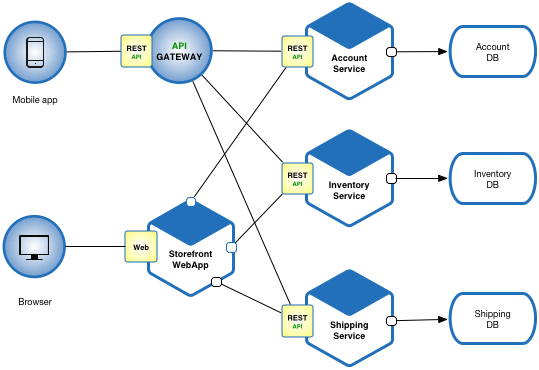
\includegraphics[scale=0.6]{images/microservices.png}
    \caption{Mikroszevizek}
    \label{fig:micro}
\end{figure}

Tehát a mikroszervizek, a nevéből értetődően kis részekből állnak, és a monolitikus rendszerek problémáit hivatottak megoldani.
Viszont ahhoz, hogy a kis, különálló szervizeket amiknek sokszor nagyon eltér a technológiai összetétele, megbízhatóan tudjuk működtetni ahhoz egy kiszámítható környezetbe kell zárni amely el van szigetelve más programoktól.
Ugyanis csak így lehet tesztelni, hogy a szoftverfüggőségek teljesülnek, és eltérő infrastruktúra alatt is működni fog az adott szervíz, alkalmazás.
Például éles és teszt környezetben eltérő infrastruktúra lehet.
De a fejlesztők dolgát is megkönnyíti ez a módszer.
Ezeket a kiszámítható környezetekhez régen virtuális gépeket használtak, de ez mára elavult, helyette konténereket használnak amelyek "könnyebbek" és jobban kihasználják az erőforrásokat.
Az alábbi diagram \ref{fig:docker-vm} mutatja a virtuális gépek és konténerek kapcsolatát.

\begin{figure}
    \centering
    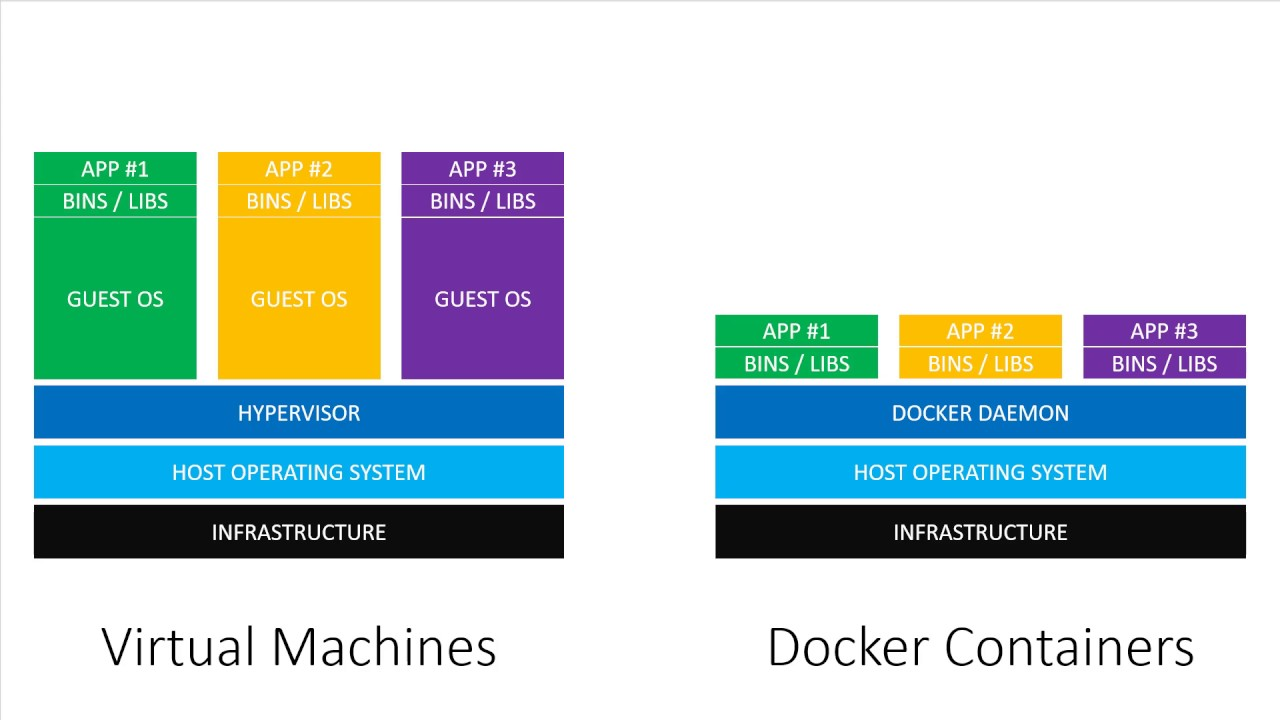
\includegraphics[scale=0.3]{images/docker-vs-vms.jpg}
    \caption{Docker konténerek és VM}
    \label{fig:docker-vm}
\end{figure}
\subsubsection{Docker}
A Docker a világ vezető szoftver konténerizáló platformja.
A megadott alkalmazást, mikroszervízt beilleszt egy úgynevezett Docker konténerbe, amelyet aztán függetlenül lehet karbantartani és telepíteni.
Hogy jobban megértsük a Docker működését nézzünk egy konkrét példát.
Egy applikációt fejleszt 3 fejlesztő, a fejlesztők rendre Windows, Mac OS-t és Linuxot használnak.
Konténerek nélkül mindegyiküknek órákon át tartó erőfeszítés lenne az alkalmazás telepítése a saját fejlesztői környezetükbe, és további erőfeszítéseket kell majd tenniük annak érdekében, hogy ugyanazt az alkalmazást később felhőbe telepítsék.
A Docker konténerek tehát egy olyan környezetet biztosítanak minden számítógépen amin fut a Docker, ami ugyanúgy működik.
Legyen szó fejlesztői, teszt vagy éles környezetről, mindig kiszámítható a működés.
A docker úgy működik, hogy egy előre meghatározott lemezből és egy bizonyos Dockerfile-ból épít egy konténert egy úgynevezett build folyamaton kereszül.
Ez a build folyamat rétegezett, azaz ha a fájlt módosítjuk, a módosítás csak az adott réteget, és az arra épülő rétegeket befolyásolja.
Így nem kell mindig újra építenünk a konténert, azt egy cache-ből előszedjük addig a rétegig, amit még nem befolyásolt a fájl módosítása.
A Dockerfileban vannak megadva a parancsok a telepítéssel kapcsolatban.
\begin{example}
    Egy konkrét példa egy egyszerű Dockerfile-ra:
    \begin{docker}
        FROM golang:1.16 AS builder
        RUN mkdir -p /go/src/drone-delivery/server
        WORKDIR /go/src/drone-delivery/server

        COPY go.mod /go/src/drone-delivery/server
        COPY go.sum /go/src/drone-delivery/server
        RUN go mod download
        COPY ./ /go/src/drone-delivery/server
        WORKDIR /go/src/drone-delivery/server/cmd/drone-delivery-server
        RUN go install

        ENTRYPOINT ["/go/bin/drone-delivery-server"]
        EXPOSE 5000
        EXPOSE 50051
    \end{docker}
\end{example}


\Section{Felhasznált eszközök}
\subsection{Architektúra, rendszer felépítése}\label{subsec:architektúra-program-felépítés}
A rendszer működésének szimulációjához 3 programot használunk ~\ref{fig:3program}.
Egy program az adatközpont, egy program a drónok szerepét veszi fel, és van még egy egyszerű böngészős web kliens amin paraméterek alapján konfigurálhatjuk a másik 2 program működését.
Az adatközpont program, és a drón-raj program a magas fokú konkurrencia kihasználásához Go nyelven készül.

\begin{figure}[h]
    \centering
    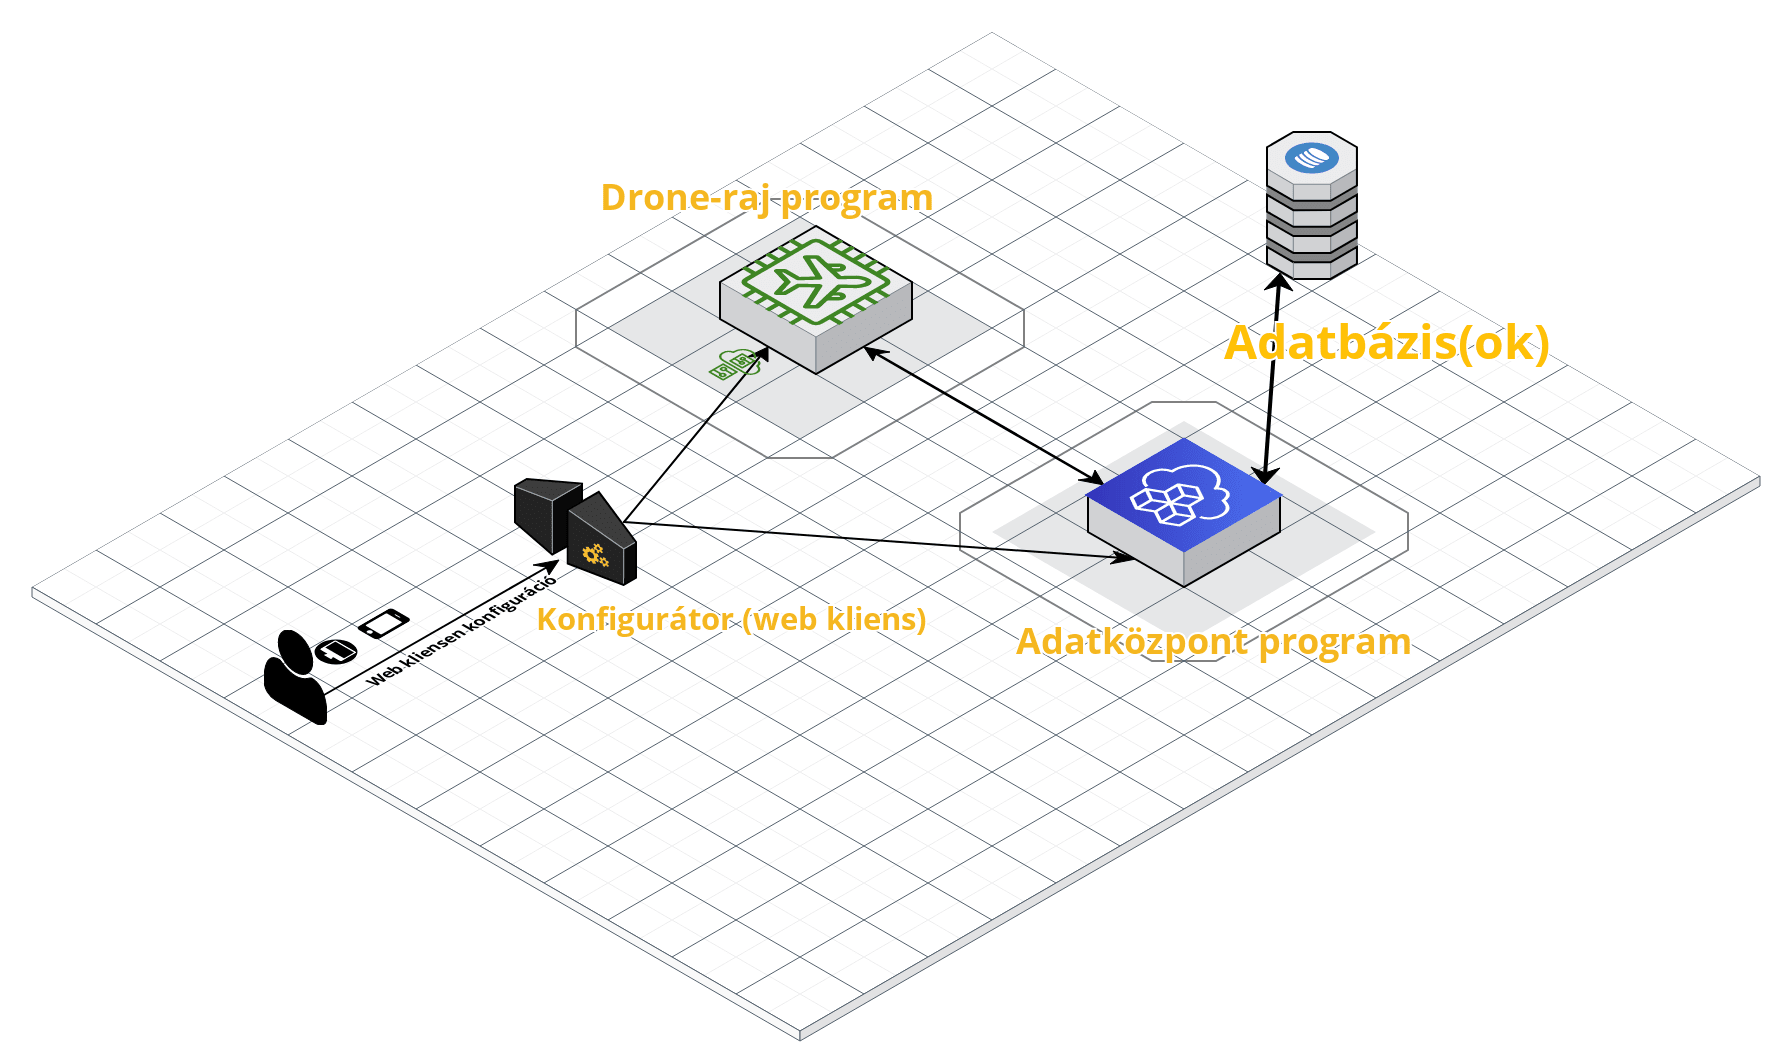
\includegraphics[scale=0.22]{images/szakdolgozat-3-program-abra.png}
    \caption{A 3 program}
    \label{fig:3program}
\end{figure}
A programoknak egymástól elszigetelt környezetben kell működniük, hogy a valódi működést megfelelően tudjuk tesztelni.
Egy számítógépen belül úgy tudjuk elérni, ha valamilyen módon konténerizáljuk a programokat, így minden program a saját elszigetelt környezetéhez fér hozzá, de a hálózaton tudnak egymással kommunikálni.
Ilyen konténerizációs szoftver a Docker.
Az adatközpontot szimuláló program lesz a legbonyolultabb.
Ennek a programnak tudnia kell elvégezni a szállítás logisztikai feladatait, valamint hatékonyan feldolgozni és tárolnia az adatokat amiket a drónok küldenek.


Ahhoz hogy a programot a követelmányben megfogalmazott módon építsük fel, értem ez alatt azt hogy több protokollt és adatbázist hasonlítsunk össze, egy olyan program architektúrát és tervezést kell választani ami megendegi ezt.
Erre a problémára megoldásként a Hexagonal (ports and adapters) architektúrát~\ref{fig:hexagonal-inward} és DDD tervezési alapelvet fogom alkalmazni.
\begin{figure}[h]
    \centering
    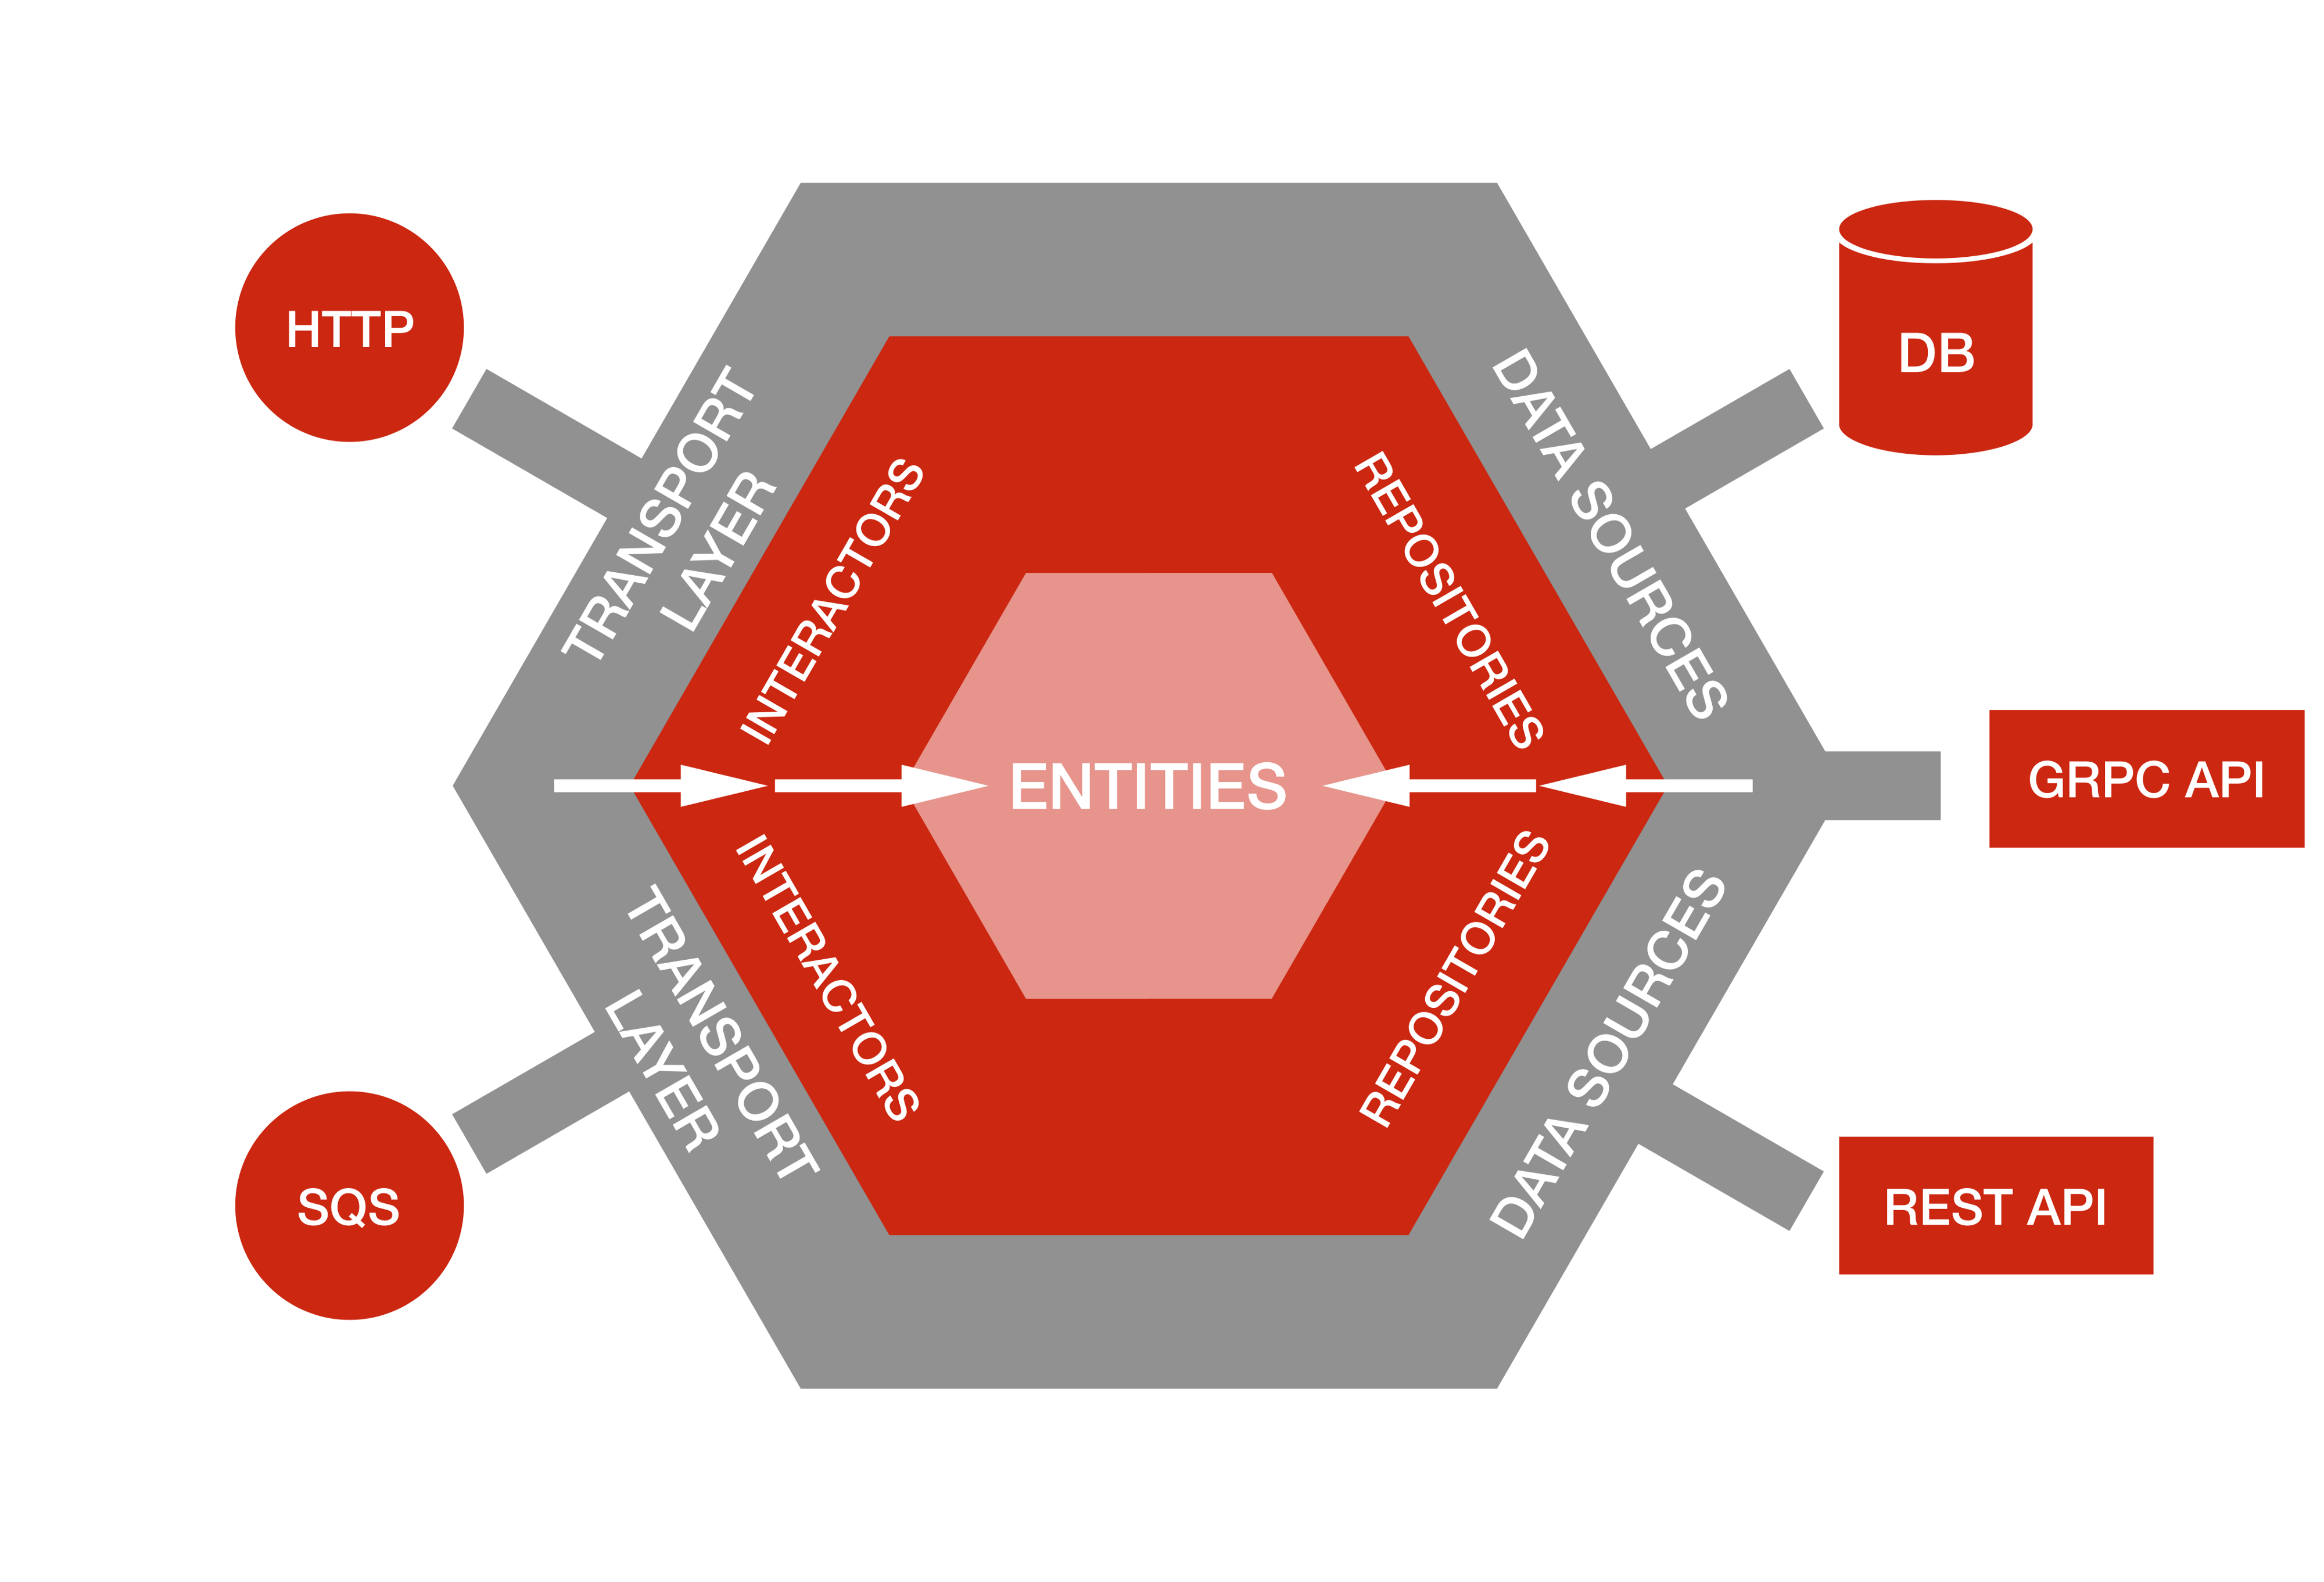
\includegraphics[scale=0.07]{images/hexa-inward.png}
    \caption{Hexagonal architecture inward pointing dependencies}
    \label{fig:hexagonal-inward}
\end{figure}

Így a program belülről kifelé epül fel, a program magja ahol az üzleti logika van interfaceket alkalmazva kommunikál a program többi részével, és nem támaszkodik semmilyen külső részre. Az intefacek miatt a külső rész a pontos implemetációja absztraktálva van, azaz csak az üzleti logikát ismerjük biztosan, minden ráépülő réteg implementációja cserélhető marad.
Minden réteg csak befelé mutat \ref{fig:hexagonal-inward}, így az üzleti logikánk megmaradhat, miközben az alkalmazás teljes infrastuktúráját kicserélhetnénk.
Így a végpontok ha teljesítik az interface elvárásait, csak dependency injection-el kicseréljük a végpontot és minden ugyanúgy működik, ám teljesen más az implementáció.
Azt hogy több fajta input és output végpontot hogy  támogatja az alkalmazás a következő ábra \ref{fig:hexagonal-inward} tökéletesen bemutatja.
Az alkalmazást fel lehet osztani verérlő és vezérelt részre. Ez nagyon jól igazodik az üzleti logikához, egy inputra szinte mindig valamiféle vezérlést várunk el,
tehát ahogz az alkalmazásunkat használjuk, vezéreljük akkor az adatok hatására valamit csináljon. Ezután az alkalmazásunk beszélhet más, külső forrásokkal, amiket az alkalmazás használ, azaz vezéreli őket.
Ilyen lehet egy adatbázis implementációja, vagy egy üzenet sor, amibe adatokat rakunk be, hogy valami más később kiolvassa.
Azért jó ez a felépítés, mert így az alkalmazásunkat több helyről meghívhatjuk, vagy felcserélhetőek ezek a helyek.
A vezérelt egységeket is ki lehet cserélni, nem vagyunk röghöz kötve mert egyszer így lett megírva az alkalmazésunk, csak a megfelelő réteget kicseréljük, feltéve hogy megírtuk hozzá az implementációnkat és az implementációnk
az intefészen keresztül teljesít minden feltételt. Így például könnyen átállhatunk relációs adatbázisról egy dokumentum alapúra, vagy egy API-t is kicserélhetünk például JSON REST API-t gRPC-re ha valami miatt szükség van rá.
A Netflix is ezt az architektúrát használja \cite{netflix}, ugyanis a gyors növekedésük közben több skálázhatósággal összefüggő problémába ütköztek, amit úgy oldottak meg hogy
ebben az architektúrában\ref{fig:hexagonal-actor} szétosztották a feladatokat több, az adott kis feladatra megfelelő adatbázisra, mikroszervízre.
\begin{figure}[h]
    \centering
    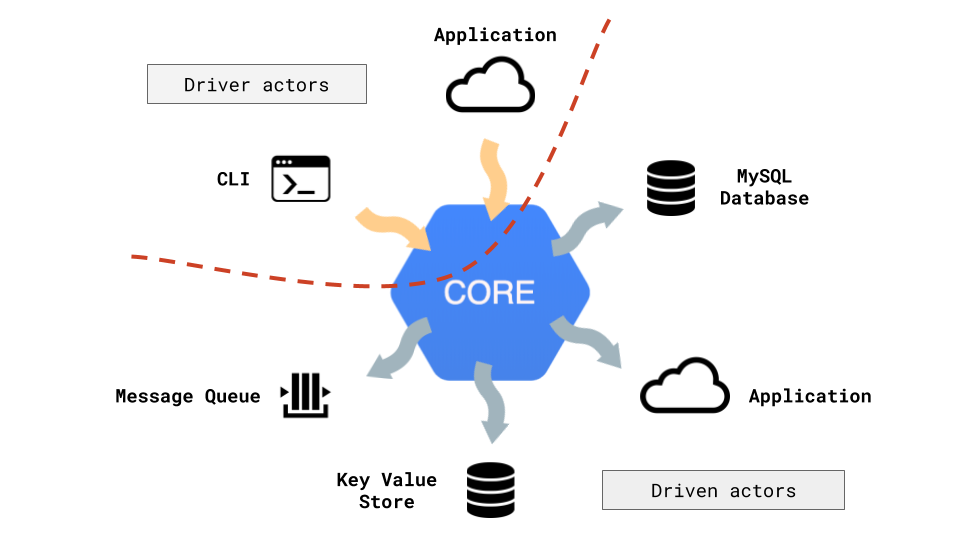
\includegraphics[scale=0.3]{images/hexa-actor.png}
    \caption{Hexagonal architecture ports and adapters}
    \label{fig:hexagonal-actor}
\end{figure}

\subsection{A Hexagonal architektúra és összehasonlítás a hagyma architektúrával}\label{subsec:a-hexagonal-architektúráról-bővebben}
A hexagonal architektúra~\cite{hexagonal}, vagy másnéven portok és adapterek architektúra a szoftver tervezés során használt design.
Célja lazán összekapcsolt alkalmazás komponensek létrehozása, amelyek portok és adapterek segítségével könnyen összekapcsolhatóak.
Ez cserélhetővé teszi a program komponenseket bármilyen szinten, és megkönnyíti a teszteket.
A működése első látszatra hasonlíthat a hagyma (réteges) architektúrához, de két külön dologról van szó.
Mindkét architektúra a Tiszta architektúra \cite{clean-architecture} elvet követi, ami arra törekszik hogy az alkalmazásunk üzleti logikája elhatárolódjon mindenféle külső környezettől, legyen az infrastruktúra, szoftver keretrendszer, user interface ami miatt ezek a tényezők cserélhetőek maradnak.
Egy fontos különbség, a hexagonal (ports and adapters) és hagyma (réteges) architektúra között, hogy a hexagonal architektúban nincsenek pontosan megnevezett rétegek, van maga a program magja ahol a domain modellek, és domain üzleti logika található, meg vannak a portok és adapterek.
A portok interfészként írhatók le, amit az adaptereknek implementálni kell, így tudnak együtt működni.
A programrészek között éles határok vannak, hiszen az adapterek nem tudnak egymásról, míg a hagyma architektúránál megengedett bizonyos "átfolyás" a rétegek között, hiszen ott a rétegek egymásra támaszkodnak és egy külső réteg használhatja bármelyik belső réteget.
Általánosságban elmondható, hogy a hexagonal architektúra sokkal modulárisabb mint a hagyma architektúra, emiatt jobban tesztelhető.
Hátránya az, hogy több kódot kell írni, így valamivel lassab nagy projekteknél.

\subsubsection{Működése részletesen}
A program magját, a domain komponenst írjuk meg először, ebbe definiáljuk az interfészeket amik a portok a külső komponensekhez.
Csak ezután kezdjük el fejlesztjük a többi komponenst.
Minden komponens nyitott egy "porton".
A komponensek közti kommunikáció ezeken a portokon történik.
A portok egy absztrak API-t definiálnak ami a megfelelő eszközzel implementálható\cite{hexagonal}.
A implementációt az adapterek valósítják meg, az objektum orientált nyelvekben interfész metódusokkal (port) vannak összekötve.


\begin{figure}[h]
    \centering
    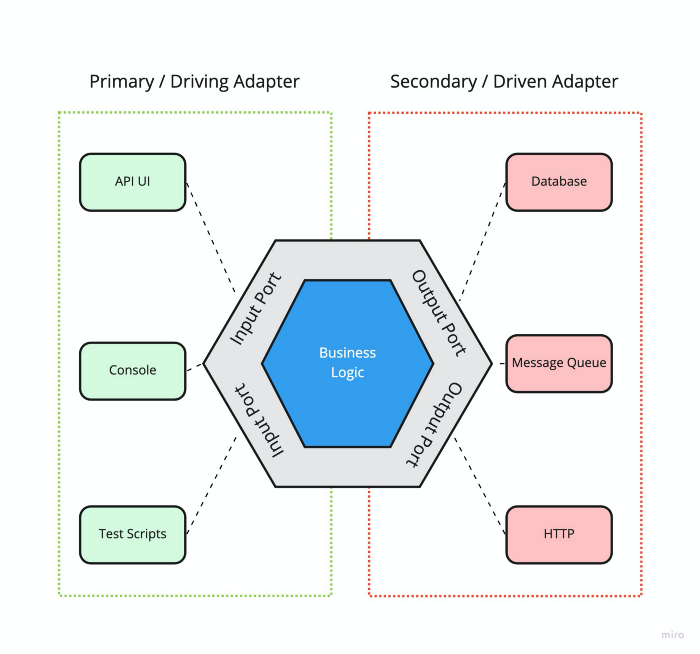
\includegraphics[scale=0.3]{images/ports-adapters}
    \caption{Hexagonal architecture driver and driven actors}
    \label{fig:hexagonal-ports-adapters}
\end{figure}

\subsection{DDD tervezési elv}
A domain vezérelt tervezés (Domain-driven design, DDD) \cite{wiki:Domain-driven_design} egy tervezési alapelv.
A koncepciója az, hogy a szoftver struktúra és kód a domain üzleti logika alapján legyen felépítve.
Tehát a jegyzék neveket, osztály neveket, metódus neveket, szervíz elnevezéseket az üzleti logikáról kell mintázni.
Tehát a program kódja az üzleti logika folyamatát követi, írja le.
Például, ha egy szoftver söröket tart nyilván, söröket lehet hozzáadni és lekérdezni, akkor olyan osztályai lehetnek mint például Beer.
Szervízt vagy valamilyen folyamatokat, műveleteket leíró absztraktot nevezhetünk el úgy mint adding, fetching.
Valamint olyan metódusok is lehetnek mint AddBeer, GetBeers.
A domain vezérelt tervezés a következő problémák megoldására használják:

\begin{itemize}
    \item A projekt középpontjában a program magja, a domain üzleti logika van.
    \item Komplex folyamatok va amik domainre épülnek.
    \item Ha magas fokú együttműködés szükséges a programozók és a domain szakértői között.
\end{itemize}

A DDD-ben vannak a domain kifejezésére, létrehozására, lekérdezésére használt sajátos artifaktok.

\begin{itemize}
    \item \textbf{\underline{Entity}}
    Olyan objektum, amit nem az attribútumai határoznak meg, hanem az identitása.
    Például, az Európai mozikban a jegy megadott székre szól, de Amerikában nincsenek megkülönböztetve a székek, egy jeggyel bárhova leülhetünk.
    Ebben az Amerikai mozi kontextusban a szék nem egy entitás, hanem egy érték objektum.
    \item \textbf{\underline{Value Object}}
    Az érték objektum egy olyan objektum amit attribútumai határoznak meg, nincs identitása.
    \item \textbf{\underline{Aggregate}}
    Objektumok csoportja, amelyeket egy gyökér entitás köt össze.
    Az aggregátumon kívüli objektumok hivatkozhatnak az aggregátum gyökerére, de más objektumára nem.
    Az aggregátum gyökere felelős az aggregátum változásainak konzisztenciájának ellenőrzéséért.
    \item \textbf{\underline{Domain Event}}
    Egy domain objektum, ami meghatároz egy esemény.
    A domain esemény egy olyan esemény, ami a domain szempontjából fontos.
    \item \textbf{\underline{Service}}
    Amikor egy művelet vagy folyamat fogalmilag nem tartozik egyetlen objektumhoz sem.
    A probléma természetes körvonalait követve ezeket a műveleteket megvalósíthatjuk a szervizekben.
    \item \textbf{\underline{Repository}}
    A domain objektumok lekérdezését egy speciális repository objektumra ruházzuk át, hogy alternatív tárolási megoldások esetén könnyen fel lehessen cserélni.
    \item \textbf{\underline{Factory}}
    A domain objektumok létrehozását egy speciális factory objektumra ruházzuk át, hogy alternatív megoldások esetén könnyen fel lehessen cserélni.
\end{itemize}

\subsubsection{Hátrányok}
Nagyon magas fokú izoláció és enkapszuláció szükséges az üzleti logikában, hogy betartsuk az összes szabályt.


\subsection{REST}\label{subsec:rest-architektúra}

A REST (Representational State Transfer) \cite{Wikipedia-REST} egy szoftverarchitektúra típus internet alapú rendszerek számára.
Egy REST architektúrának meg kell felelni a következő megszorításoknak:
\begin{itemize}
    \item Kliens-szerver architektúra
    \item Állapotmentesség
    \item Gyorsítótárazhatóság
    \item Réteges felépítés
    \item Egységes interfész
\end{itemize}

\subsubsection{Kliens-szerver architektúra}
A kliensek egy egységes interfészen keresztül beszélnek.
Az érdekeltségek ilyen nemű szétválasztása azt jelenti, például, hogy a kliensek nem foglalkoznak adattárolással, ami a szerver belső ügye marad, és így a kliens kód hordozhatósága megnő.
A szerverek nem foglalkoznak a felhasználói felülettel vagy a kliens állapotával, így a szerverek egyszerűbbek és még skálázhatóbbak lehetnek.
A szerverek és kliensek áthelyezhetőek és fejleszthetőek külön-külön is, egészen addig amíg az interfész nem változik meg.
\subsubsection{Állapotmentesség}
A kliens-szerver kommunikáció tovább korlátozott az által, hogy a szerveren nem tárolják a kliens állapotát a kérések között.
Minden egyes kérés bármelyik klienstől tartalmazza az összes szükséges információt a kérés kiszolgálásához, és minden állapotot a kliens tárol.
\subsubsection{Gyorsítótárazhatóság}
Mint ahogy a világhálón, a kliensek itt is képesek gyorsítótárazni a válaszokat.
A válaszoknak ezért impliciten vagy expliciten tartalmazniuk kell, hogy gyorsítótárazhatóak-e vagy sem.
Egy jól menedzselt gyorsítótár lehetővé teszi, hogy teljesen megkerüljünk egyes kliens-szerver interakciókat, továbbá megnöveli a rendszer skálázhatóságát és a teljesítményét.
\subsubsection{Réteges felépítés}
Egy kliens általában nem tudja megmondani, hogy direkt csatlakozott-e a végpont szerverhez, vagy közvetítő segítségével.
A közvetítő szerverek megnövelhetik a rendszer skálázhatóságát terheléseloszlással és gyorsítótárak használatával.
\subsubsection{Egységes interfész}
Az egységes interfész kliens és szerver között egyszerűsíti és kettéválasztja az architektúrát, és lehetővé teszi, hogy egymástól függetlenül fejlődjenek az egyes részek.


Ha ezeket a megkötéseket teljesíti a webes szolgáltatásunk, azt mondhatjuk hogy "RESTful".


\subsubsection{A REST működése}
A kliensek kéréseket indítanak a szerverek felé, a szerverek pedig feldolgozzák a kéréseket és egy választ küldenek vissza.
A kérések és a válaszok erőforrás reprezentációk köré épülnek.
Ezek az erőforrás reprezentációk a mi esetünkben JSON dokumentumok.
Az erőforrásokat az URL címével és a HTTP metódussal azonosítjuk.
A következő példában láthatjuk ahogy egy PUT metódussal és az URL-ben megadott paraméterrel pontosan tudjuk azonosítani mit szeretnénk.
A PUT requestet akkor használjuk ha egy már meglévő erőforrást szeretnénk felülírni, esetünkben az adatbázis konfigurációt kicseréljük.
A :name paraméter pedig megnevezi az erőforrást amire a meglévőt ki szeretnénk cserélni.
Válaszként egy JSON dokumentumot küldünk vissza válaszként a megfelelő státuszkóddal, hogy a kérés sikeres volt vagy sem.

\begin{python}
    router.PUT("/configure/database/:name", func(c echo.Context) error {
        switch c.Param("name") {
            case "mongodb":
            t.ChangeService(m)
            d.ChangeService(m)
            case "postgres":
            t.ChangeService(p)
            d.ChangeService(p)
            default:
            return echo.NewHTTPError(
            http.StatusBadRequest,
            "no such database supported"
            )
        }
        return c.JSON(http.StatusOK, "configuration complete")
    })
\end{python}


\subsection{HTTP/2 gRPC összehasonlítása HTTP/1.1 JSON üzenetváltással}

\paragraph{REST és HTTP 1.1, JSON üzenetváltás}
A mikroszevízes infrastuktúra egy nagyon elterjedt módja az elosztott rendszerek tervezésének.
Sok mikroszervíz a mai napig REST API-n kommunikál, HTTP 1.1-es protokollon keresztül és JSON dokumentumokat küldenek és fogadnak.
Ez a megoldás a fejlesztőknek kedvez, nagyon egyszerű így fejleszteni manapság, rengeteg eszköz van hogy megyorsítsa és megkönnyítse a munkánkat.
De ez a megoldás a teljesítmény rovására megy, ugyanis a következő problémák adódnak vele:
\begin{itemize}
    \item A HTTP/1.1  szöveg alapú és nagyon "nehéz". A kommunikáció hatalmas adatmennyiséget igényel, ez egy felesleges teher.
    \item A HTTP/1.1  állapotmentes, ezért az állapotokat csak a fejlécben tudjuk jelezni, ami nem tömörített.
    \item A HTTP/1.1  unáris - azaz - egy kérésre egy választ kapsz. Nem lehet egyszerre több kérdést küldeni, minden kérésre pontosan egy válasz jön.
    \item Minden egyes HTTP/1.1 kéréshez 3 irányú üzenet váltáshoz van szükség, csak hogy létrehozzuk a TCP kapcsolatot, mivel a TCP kapcsolat full duplex, és mindkét fél szinkronizálja és nyugtázza egymást.
\end{itemize}
Ebből arra következtetünk, hogy olyan szerver és szerver közötti kommunikációra ahol viszonylag sok apró kérés van, vagy a fenti problémák
akadályozzák a programunk működését, akkor érdemes más megoldások után néznünk.

\subsection{RPC}
Az RPC \cite{RPC} (Remote Procedure Call) egy szabvány, olyan távoli eljárás hívás amelynek segítségével használni lehet egy, ugyanabban a hálózatban található távoli gépen futó programot anélkül, hogy a hálózati részletekkel foglalkozni kellene.
Az RPC a kliens/szerver modellt használja (a kérő a kliens, a programot futtató fél a szerver).

\subsection{gRPC}
A gRPC \cite{gRPC} egy Google által fejlesztett RPC keretrendszer, főleg mikroszervizek közötti kommunikációra.
A gRPC HTTP/2-t használ és Protocol Buffert az üzenetváltáshoz JSON helyett. Ez szembemegy a megszokott mikroszervizes architektúra stílussal ami REST-re épül JSON üzenetváltásal HTTP/1.1-en.
Triviális, hogy a legfontosabb előnye az, hogy HTTP/2-n fut és az üzenetváltás Protocol Bufferekkel történik így sokkal gyorsabb és hatékonyabb.


\paragraph{HTTP/1.1 és HTTP/2 összehasonlítása}
A HTTP/2 egy sokkal hatékonyabb protokoll, a streameléssel elérhetjük azt, hogy az egyik fél több üzenetet is küld, a másik fél viszont csak a kérések legvégén válaszol.
\begin{table}[h]
    \centering
    \caption{HTTP/1.1 és HTTP/2}
    \label{tab:http}
    \begin{tabular}{|c|c|}
        \hline
        HTTP/1.1 & HTTP/2 \\
        \hline
        Szöveges formátum & Bináris formátum \\
        \hline
        Szöveges, nem tömörített fejléc & Tömörített fejléc \\
        \hline
        1 kérés, 1 válasz TCP kapcsolatonként & 1 TCP kapcsolatot újra felhasználunk,\\
        & Unáris kérések,\\
        & Szerver streamelés,\\
        & Kliens streamelés,\\
        & Két-irányú streamelés\\
        \hline
    \end{tabular}
\end{table}

\paragraph{Protocol Buffer és JSON összehasonlítása}

Beláthatjuk, hogy a Protocol Buffer adatforgalom kontextusban és hardveres erőforrás kontextusban is egy sokkal hatékonyabb eszköz üzenetek továbbítására mint a JSON, XML, stb hagyományos formátumok.
Mivel nem szöveges, lehet hogy nehezebb implementálni és debugolni a fejlesztőknek, viszont kevesebb adatforgalommal jár, és a számítógép erőforrásait is kíméli, nem úgy mint a JSON.

\begin{table}[h]
    \centering
    \caption{JSON és Protocol Buffer}
    \label{tab:message-exchange}
    \begin{tabular}{|c|c|}
        \hline
        JSON & Protocol Buffer \\
        \hline
        Nincs szigorú séma definíció & Szigorú séma formátum \\
        vagy típus & és típus biztonság \\
        \hline
        Szöveg alapú & Bináris \\
        \hline
        A szöveg formátum miatt lassú & Bináris formátum miatt gyors\\
        szérializáció és deszérializáció & szérializáció és deszérializáció\\
        CPU és memória intenzív & \\
        \hline
        Adatok manuális konvertálása & Generált kód a protokol buffer séma alapján\\
        \hline
    \end{tabular}
\end{table}

\subsection{Adatbázisok}
Az adatok adatbázisba mentése, adatbázisból olvasása közben több probléma merülhet fel, a rendszer konkurrens felépítéséből kiindulva.
Például amikor az épp szabad drónoknak adunk feladatot, lehet hogy 2 vagy több egyede az adatközpont programunknak kiolvassa azt az értéket hogy a drón nem csinál semmit, az állapota szabad, adhat neki feladatot ha van szállítsra váró csomag.
De, az üzleti logika futtatása közben az egyik egyed módosíthatta
az értéket arra hogy már repül, vagy épp csomagot vesz fel.
Az ilyen Lost Update problémákkal szemben védelmet ad, ha az adatbázis rendelkezik ACID tulajdonságokkal.
Az ACID tulajdonságok \ref{fig:acid} (atomiság, konzisztencia, izoláció, tartósság) felelősek az adatbázis integritásáért.

\begin{figure}[h]
    \centering
    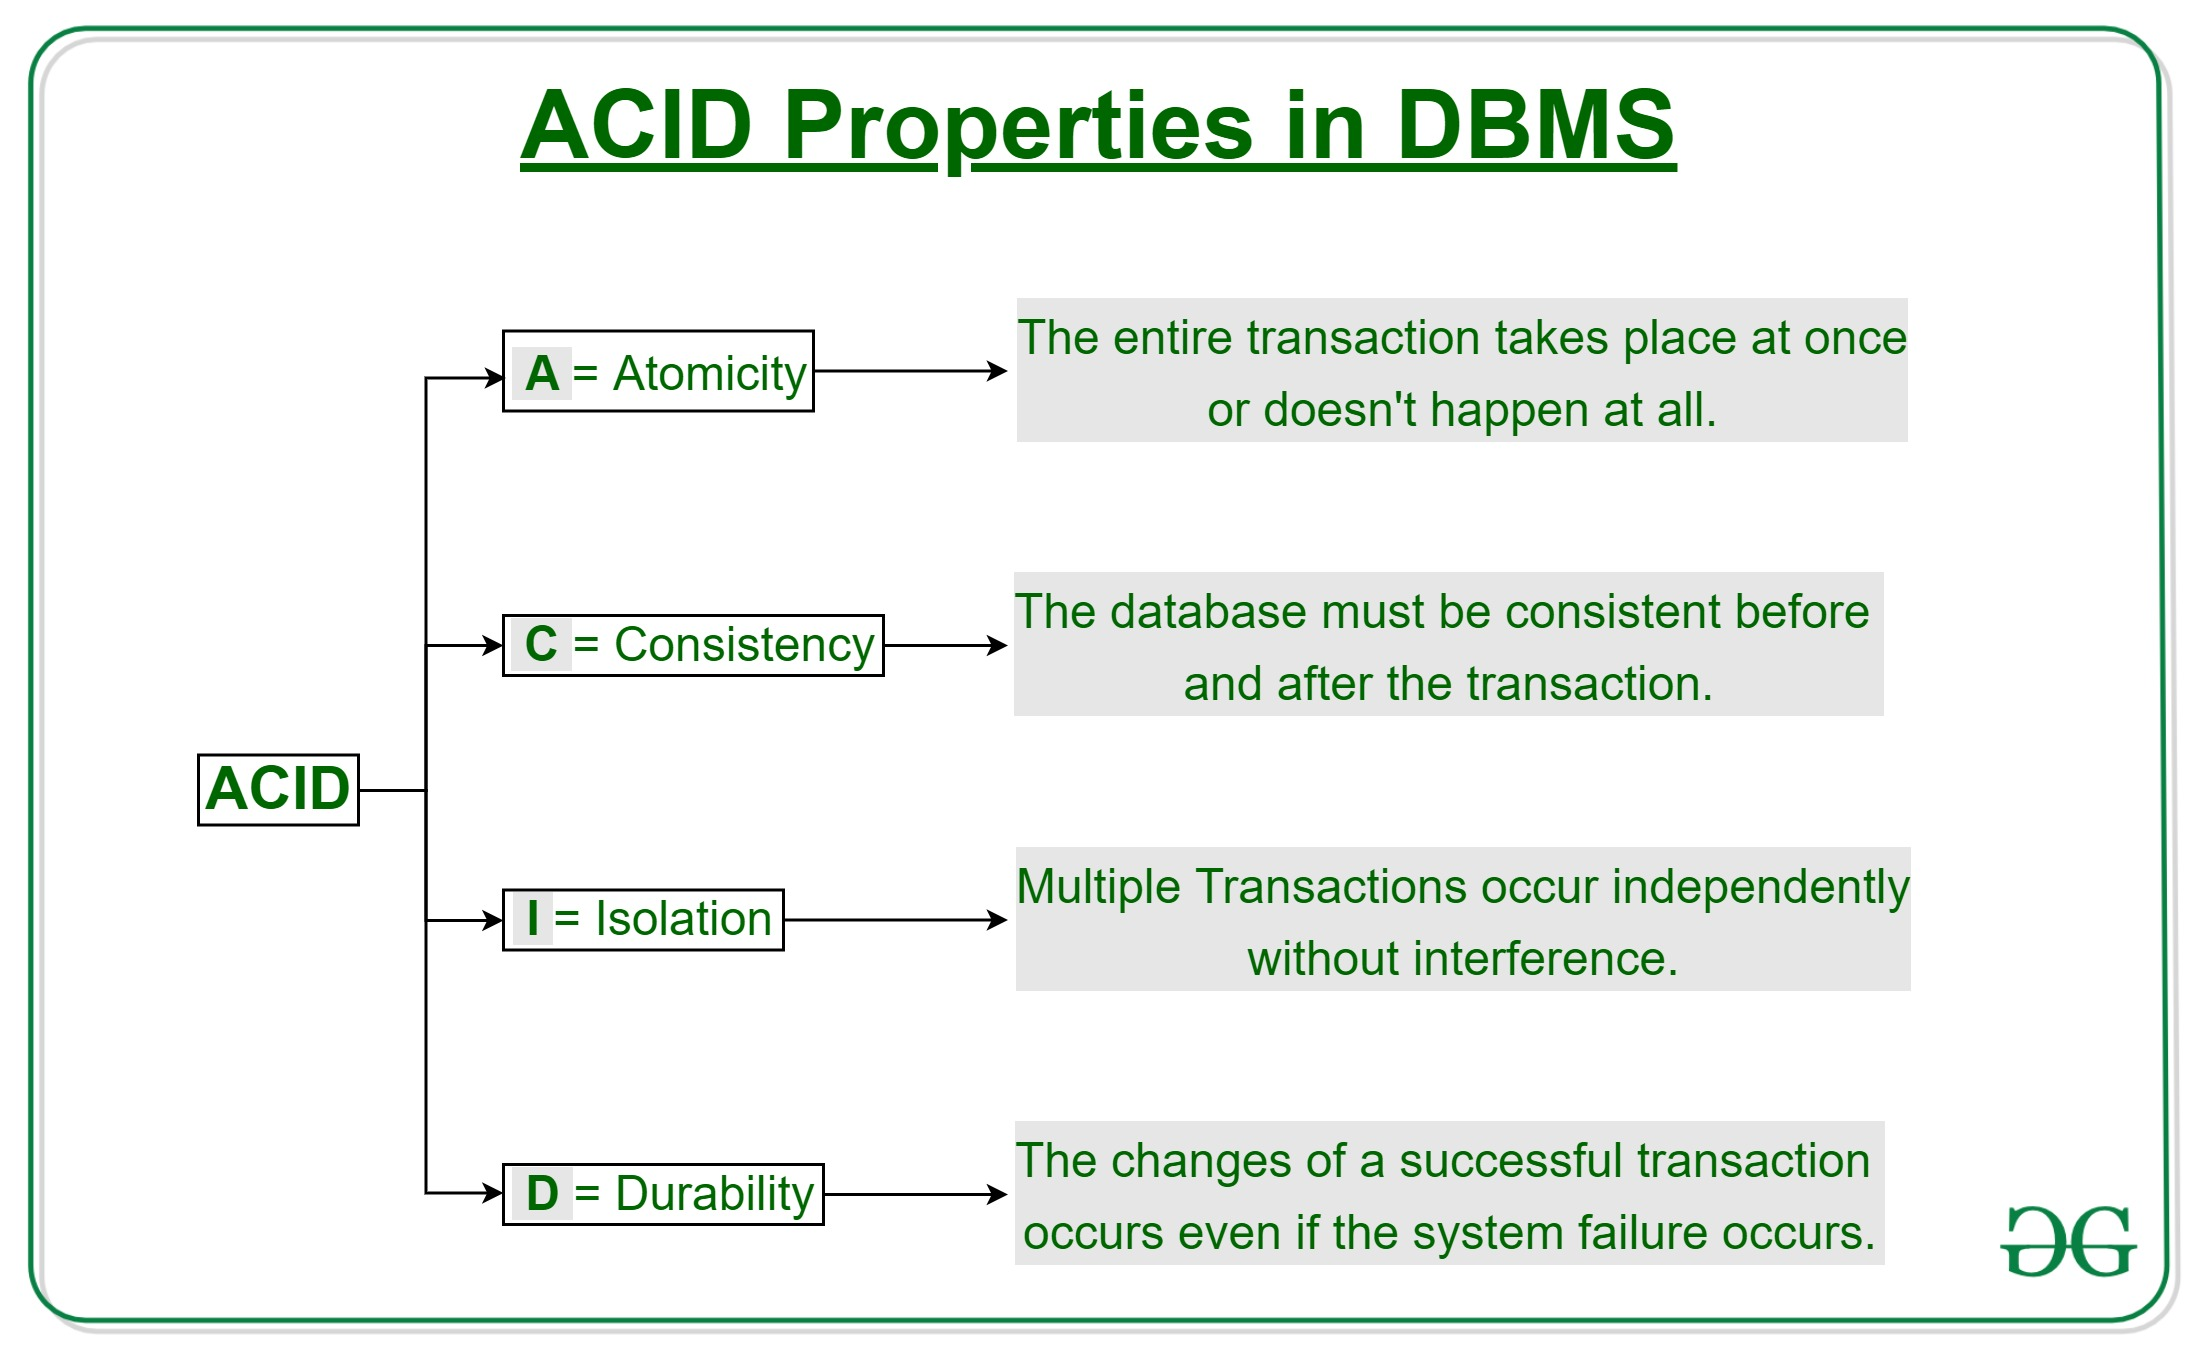
\includegraphics[scale=0.15]{images/ACID-Properties.jpg}
    \caption{ACID tulajdonságok}
    \label{fig:acid}
\end{figure}

Tehát csak olyan adatbázisok jöhetnek szóba a program implementálásánál aminek az integritása garantálható.
Hogy 2 eltérő adatbázist hasonlítsunk össze, egy SQL és egy NoSQL adatbázis ami teljesíti az ACID integritást megfelelő lesz.
A PostgreSQL adatbázis kíváló relációs adatbázis, nem véletlen, hogy az egyik legelterjedtebb. Teljesíti az ACID tulajdonságokat, és már 35 éve használják így biztosan megfelelően tesztelt.
A MongoDB dokumentum alapú adatbázis ACID, de csak dokumentum szintent. A mi szimulációnkhoz viszont így is megfelel a követelményeknek.
Érdekességként, a legtöbb dokumentum alapú adatbázis nem ACID, ezért nem annyira népszerűek.
A dokumentum alapú adatbázisok általában jobban teljesítenek ha nagyon sok írás történik lekérdezés pedig kevés, vagy ha nincs bonyolult lekérdezés ami több JOIN-t igényel.

\subsection{Protokollok és adatbázisok szerepe a programban}
A drón raj programot és az adatközpontot úgy tervezzük meg, hogy a telemetria adatok küldéséhez használt rész kicserélhető legyen valamilyen módon (például dependency injekción keresztül).
Így tudjuk összehasonlítani a több protokollon keresztüli kommunikációt. Az adatbázis végpontot is hasonlóan ki kell tudnunk cserélni, hogy ne kelljen módosítani a programon a különböző szimulációkhoz.
A következő kód példában láthatjuk, hogy működhet a dependency injekció. Itt a postgreSQL adatbázissal hoztuk létre a szervízt, de a mongoDB adatbázissal is létrehozhatjuk, ha teljesíti az interfész követelményeit.
\begin{python}
    postgresStorage, err := postgres.NewStorage(config.PostgresConfig)
    if err != nil {
        log.Println("Error connecting to database")
        panic(err)
    }
    mongoStorage, err := mongodb.NewStorage(config.MongoConfig)
    if err != nil {
        log.Println("Error connecting to database")
        panic(err)
    }
    var ts telemetry.Service
    var ds drone.Service
    var rs routing.Service
    ts = telemetry.NewService(postgresStorage, logger)
    rs = routing.NewService(logger)
    ds = drone.NewService(postgresStorage, jsonAdapter, logger, rs)
\end{python}




